% \iffalse
\let\negmedspace\undefined
\let\negthickspace\undefined
\documentclass[journal,12pt,twocolumn]{IEEEtran}
\usepackage{cite}
\usepackage{amsmath,amssymb,amsfonts,amsthm}
\usepackage{algorithmic}
\usepackage{graphicx}
\usepackage{textcomp}
\usepackage{xcolor}
\usepackage{txfonts}
\usepackage{listings}
\usepackage{enumitem}
\usepackage{mathtools}
\usepackage{gensymb}
\usepackage{comment}
\usepackage[breaklinks=true]{hyperref}
\usepackage{tkz-euclide} 
\usepackage{listings}
\usepackage{gvv}  
\usepackage{tikz}
\usepackage{circuitikz} 
\usepackage{caption}

\def\inputGnumericTable{}                                
\usepackage[latin1]{inputenc}                 
\usepackage{color}                            
\usepackage{array}                            
\usepackage{longtable}                        
\usepackage{calc}                            
\usepackage{multirow}                      
\usepackage{hhline}                           
\usepackage{ifthen}                          
\usepackage{lscape}
\usepackage{amsmath}
\newtheorem{theorem}{Theorem}[section]
\newtheorem{problem}{Problem}
\newtheorem{proposition}{Proposition}[section]
\newtheorem{lemma}{Lemma}[section]
\newtheorem{corollary}[theorem]{Corollary}
\newtheorem{example}{Example}[section]
\newtheorem{definition}[problem]{Definition}
\newcommand{\BEQA}{\begin{eqnarray}}
\newcommand{\EEQA}{\end{eqnarray}}
\newcommand{\define}{\stackrel{\triangle}{=}}
\theoremstyle{remark}
\newtheorem{rem}{Remark}

\begin{document}
\title{Gate Assignment CH 31}
\author{Shravya Kantayapalam\\ EE23BTECH11030}
\maketitle

\begin{enumerate}
    \item \textbf{Question }:
The position \( x(t) \) of a particle, at constant \( \omega \), is described by the equation
\[
\frac{{d^2x}}{{dt^2}} = -\omega^2 x.
\]
The initial conditions are \( x(t=0) = 1 \) and \( \frac{{dx}}{{dt}}\bigg|_{t=0} = 0 \). 

The position of the particle at \( t = \frac{{3\pi}}{{\omega}} \) is \underline{\hspace{2cm}} (in integer).
\hfill{(GATE CH 2023)}

\solution

\begin{table}[htbp]
    \centering
    \caption{Input Parameters}
    \begin{tabular}{|c|c|}
        \hline
        \textbf{Parameter} & \textbf{Description} \\
        \hline
        $s$ & Complex frequency variable in Laplace domain \\
        $\omega$ & Angular frequency \\
        $X(s)$ & Laplace transform of the function $x(t)$ \\
        $x(t)$ & Time-domain function \\
        \hline
    \end{tabular}
\end{table}

\[
s^2X(s) - sx(0) - \frac{{dx}}{{dt}}(0) + \omega^2X(s) = 0
\]

\[
x(0) = 1 \quad \text{and} \quad \frac{{dx}}{{dt}}(0) = 0
\]

\[
s^2X(s) - s - \omega^2X(s) = 0
\]

\[
(s^2 + \omega^2)X(s) = s
\]

\[
X(s) = \frac{{s}}{{s^2 + \omega^2}}
\]

\[
X(s) = \frac{{s}}{{s^2 + \omega^2}} = \frac{{A}}{{s}} + \frac{{Bs + C}}{{s^2 + \omega^2}}
\]

Multiplying both sides by $s(s^2 + \omega^2)$, we get:
\[
s = A(s^2 + \omega^2) + (Bs + C)s
\]

This implies $A = 0$, $B = 1$, and $C = 0$. Therefore,
\[
X(s) = \frac{{1}}{{s^2 + \omega^2}}
\]

\[
x(t) = \mathcal{L}^{-1} \left\{ \frac{{1}}{{s^2 + \omega^2}} \right\} = \cos(\omega t)
\]

Finally, evaluating $x(t)$ at $t = \frac{{3\pi}}{{\omega}}$, we have:
\[
x\left(\frac{{3\pi}}{{\omega}}\right) = \cos\left(\omega \cdot \frac{{3\pi}}{{\omega}}\right) = \cos(3\pi) = -1
\]
\begin{figure}[ht]
    \centering
    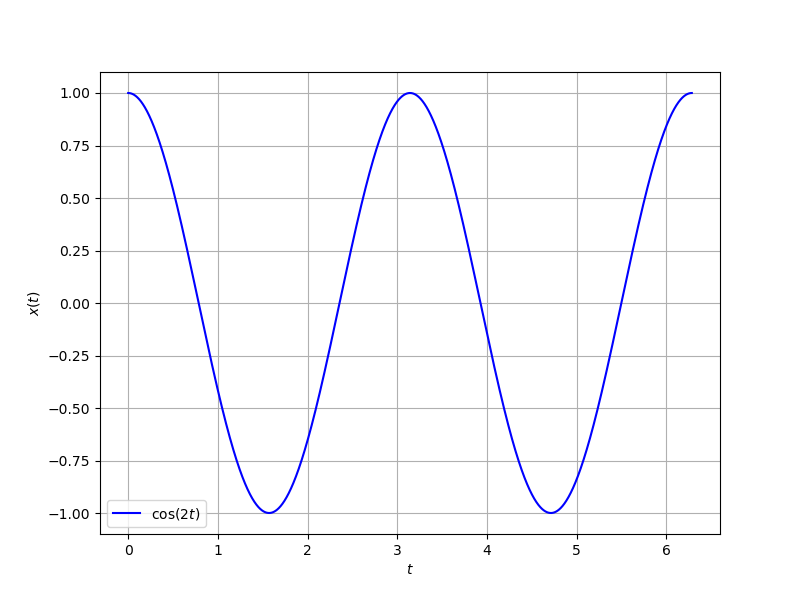
\includegraphics[width=\columnwidth]{gate.png}
    \caption{Graph of $x(t)$}
\end{figure}
\end{document}


